\section{Das Sechs-Inkreise-Lemma}\label{kapitel:SechsInkreise}
In diesem Kapitel werdet ihr ein Lemma kennenlernen, das sich immer dann anwenden lässt, wenn in einer Aufgabe ein Tangentenviereck sowie mehrere weitere Inkreise vorkommen. Die Nützlichkeit dieses Lemmas werden wir an zwei Beispielaufgaben demonstrieren. Am Ende des Kapitels findet ihr Tipps zu den Aufgaben und am Ende des Heftes könnt ihr die Lösungen nachschlagen. Bevor ihr euch die Lösungen durchlest, solltet ihr aber auf jeden Fall versuchen, die Aufgaben (mit den Tipps) selbstständig zu lösen.
\begin{aufgabe*}\label{aufgabe:SechsInkreiseSehnenviereck}
	Sei $ABCD$ ein Tangentenviereck und $P$ ein innerer Punkt der Strecke $\overline{CD}$. Die Inkreismittelpunkte der Dreiecke $DAP$, $ABP$ und $BCP$ seien mit $I$, $J$ und $K$ bezeichnet. Beweise, dass $PIJK$ ein Sehnenviereck ist.
\end{aufgabe*}
\begin{aufgabe*}\label{aufgabe:531246}
	Sei $ABCD$ ein Tangentenviereck mit Inkreismittelpunkt $I$. Auf den Strecken $\overline{AI}$ und $\overline{CI}$ liegen Punkte $P$ und $Q$, sodass $\winkel QBP=\frac12\winkel CBA$ gilt. Zeige, dass dann auch $\winkel PDQ=\frac 12\winkel ADC$ gilt.
\end{aufgabe*}

Kommen wir nun zu dem Lemma, dem dieses Kapitel gewidmet ist. Bevor ihr euch den Beweis durchlest, solltet ihr versuchen, das Lemma selbst zu beweisen, denn das ist eine gute Übungsaufgabe.
\begin{satzmitnamen}[Sechs-Inkreise-Lemma]
	Wenn in der folgenden Skizze fünf der sechs eingezeichneten Inkreise $\omega_A$, $\omega_B$, $\omega_C$, $\omega_D$, $\omega$ und $\Omega$ existieren, dann existiert auch der sechste Inkreis.
\end{satzmitnamen}
\begin{figure}[ht]
	\centering
	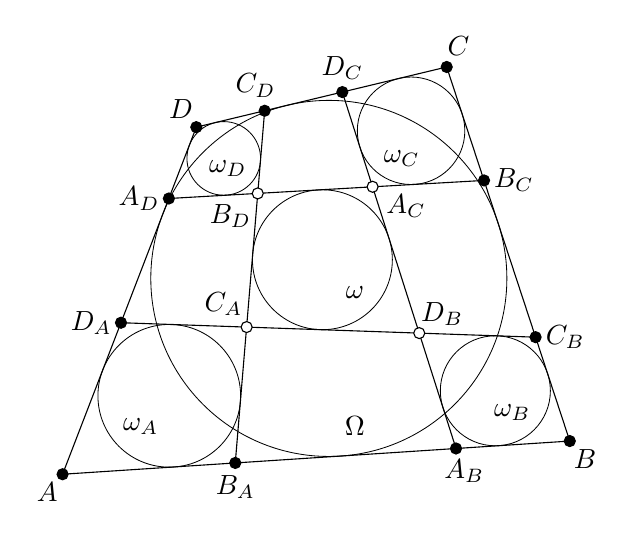
\begin{tikzpicture}[x=0.85cm,y=0.85cm]
		\draw [line width=0.3] (-10.79,11.71) circle (2.66);
		\draw [line width=0.3] (-10.886,11.989) circle (1.045);
		\draw [line width=0.3] (-12.36,13.503) circle (0.55);
		\draw [line width=0.3] (-9.561,13.916) circle (0.803);
		\draw [line width=0.3] (-13.174,9.956) circle (1.066);
		\draw [line width=0.3] (-8.302,10.031) circle (0.822);
		\coordinate (A) at (-14.768,8.784);
		\coordinate (B) at (-7.19,9.28);
		\coordinate (C) at (-9.029,14.869);
		\coordinate (D) at (-12.77,13.97);
		\coordinate (Ba) at (-12.188,8.953);
		\coordinate (Ca) at (-12.018,10.983);
		\coordinate (Da) at (-13.895,11.048);
		\coordinate (Ab) at (-8.89,9.169);
		\coordinate (Cb) at (-7.701,10.832);
		\coordinate (Db) at (-9.439,10.893);
		\coordinate (Ac) at (-10.136,13.079);
		\coordinate (Bc) at (-8.471,13.174);
		\coordinate (Dc) at (-10.588,14.494);
		\coordinate (Ad) at (-13.18,12.904);
		\coordinate (Bd) at (-11.852,12.98);
		\coordinate (Cd) at (-11.749,14.215);
		\draw (A) to (B) to (C) to (D) to cycle;
		\draw (Ba) to (Cd);
		\draw (Ab) to (Dc);
		\draw (Da) to (Cb);
		\draw (Ad) to (Bc);
		\draw[fill=black] (A) circle (2pt) node[shift={(230:2ex)}] {$A$};
		\draw[fill=black] (Ab) circle (2pt) node[shift={(290:2ex)}] {$A_B$};
		\draw[fill=white] (Ac) circle (2pt) node[shift={(330:3.25ex)}] {$A_C$};
		\draw[fill=black] (Ad) circle (2pt) node[shift={(180:2.5ex)}] {$A_D$};
		\draw[fill=black] (B) circle (2pt) node[shift={(310:2ex)}] {$B$};
		\draw[fill=black] (Ba) circle (2pt) node[shift={(270:2ex)}] {$B_A$};
		\draw[fill=black] (Bc) circle (2pt) node[shift={(0:2.5ex)}] {$B_C$};
		\draw[fill=white] (Bd) circle (2pt) node[shift={(220:3ex)}] {$B_D$};
		\draw[fill=black] (C) circle (2pt) node[shift={(60:2ex)}] {$C$};
		\draw[fill=white] (Ca) circle (2pt) node[shift={(135:2.75ex)}] {$C_A$};
		\draw[fill=black] (Cb) circle (2pt) node[shift={(0:2.5ex)}] {$C_B$};
		\draw[fill=black] (Cd) circle (2pt) node[shift={(110:2.25ex)}] {$C_D$};
		\draw[fill=black] (D) circle (2pt) node[shift={(130:2ex)}] {$D$};
		\draw[fill=black] (Da) circle (2pt) node[shift={(180:2.5ex)}] {$D_A$};
		\draw[fill=white] (Db) circle (2pt) node[shift={(40:2.5ex)}] {$D_B$};
		\draw[fill=black] (Dc) circle (2pt) node[shift={(90:2ex)}] {$D_C$};
		\node at (-13.6,9.5) {$\omega_A$};
		\node at (-8.05,9.7) {$\omega_B$};
		\node at (-9.7,13.5) {$\omega_C$};
		\node at (-12.3,13.35) {$\omega_D$};
		\node at (-10.4,11.5) {$\omega$};
		\node at (-10.4,9.5) {$\Omega$};
	\end{tikzpicture}
\end{figure}

\begin{proof}
	Um nicht 16 verschiedene Berührpunkte benennen zu müssen, führen wir die folgende Nichtstandardnotation ein: Für zwei Kreise $\Omega_1$ und $\Omega_2$, die nicht ineinander liegen, sei $\abs{\Omega_1\Omega_2}$ die Länge der Strecke zwischen den Berührpunkten einer gemeinsamen äußeren Tangenten von $\Omega_1$ und $\Omega_2$. Da Punkte Kreise mit Radius $0$ sind, weitet sich die Notation auf den Fall aus, dass $\Omega_1=\{X\}$ ein Punkt ist. In diesem Fall ist $\abs{X\Omega_2}$ die Länge eines Tangentenabschnitts von $X$ an $\Omega_2$. Und falls $\Omega_2=\{Y\}$ selber ein Punkt ist, erhalten wir mit $\abs{XY}$ unsere Standardnotation für Streckenlängen zurück.
	
	Wir nehmen zunächst an, dass die Kreise $\omega_A$, $\omega_B$, $\omega_C$ und $\omega_D$ existieren. Wir wollen zeigen, dass $ABCD$ genau dann ein Tangentenviereck ist, wenn $A_CB_DC_AD_B$ ein Tangentenviereck ist. Mit der obigen Notation gilt $\abs{AB}=\abs{A\omega_A}+\abs{\omega_A\omega_B}+\abs{\omega_BB}$. Analoge Gleichungen gelten auch für die Seiten $\overline{BC}$, $\overline{CD}$ und $\overline{DA}$. Also ist
	\begin{equation*}
		\abs{AB}+\abs{CD}-\abs{BC}-\abs{DA}=\abs{\omega_A\omega_B}+\abs{\omega_C\omega_D}-\abs{\omega_B\omega_C}-\abs{\omega_D\omega_A}\,,
	\end{equation*}
	denn die Tangentenabschnitte $\abs{A\omega_A}$, $\abs{B\omega_B}$, $\abs{C\omega_C}$ und $\abs{D\omega_D}$ heben sich gerade weg. Völlig analog gilt $\abs{A_CB_D}=\abs{\omega_C\omega_D}-\abs{B_D\omega_D}-\abs{A_C\omega_C}$ und entsprechende Gleichungen für die anderen Seiten. Wir erhalten also 
	\begin{equation*}
		\abs{A_CB_D}+\abs{C_AD_B}-\abs{B_DC_A}-\abs{D_BA_C}=\abs{\omega_A\omega_B}+\abs{\omega_C\omega_D}-\abs{\omega_B\omega_C}-\abs{\omega_D\omega_A}\,.
	\end{equation*}
	Aus diesen Gleichungen folgt:
	\begin{align*}
		\abs{AB}+\abs{CD}=\abs{BC}+\abs{DA}&\Longleftrightarrow \abs{\omega_A\omega_B}+\abs{\omega_C\omega_D}=\abs{\omega_B\omega_C}+\abs{\omega_D\omega_A}\\
		&\Longleftrightarrow \abs{A_CB_D}+\abs{C_AD_B}=\abs{B_DC_A}+\abs{D_BA_C}\,.
	\end{align*}
	Mit anderen Worten: $ABCD$ ist ein Tangentenviereck genau dann, wenn $A_CB_DC_AD_B$ eines ist, sprich $\omega$ existiert genau dann, wenn $\Omega$ existiert.
	
	Jetzt nehmen wir an, dass $\omega$, $\Omega$ sowie drei der vier Kreise $\omega_A$, $\omega_B$, $\omega_C$ und $\omega_D$ existieren. Sei o.B.d.A.\ $\omega_A$ der fehlende. Sei $\omega_A'$ der Kreis, der die Strecken $\overline{AD}$, $\overline{AB_A}$ und $\overline{B_AC_D}$ berührt und sei $\ell$ die von $AB$ verschiedene gemeinsame äußere Tangente von $\omega_A'$ und $\omega_B$. Nach dem Teil, den wir schon bewiesen haben, muss $\ell$ auch den Kreis $\omega$ tangieren. Dann ist aber $\ell$ identisch mit der Geraden $D_AC_B$! Folglich ist $\omega_A'$ der Inkreis von $AB_AC_AD_A$, und insbesondere existiert der Inkreis $\omega_A=\omega_A'$.
\end{proof}

Das Sechs-Inkreise-Lemma ist insbesondere dann nützlich, wenn einige der kleinen Vierecke zu Punkten degenerieren (sodass ihre Inkreise aus trivialen Gründen existieren). Macht euch an Beispielen klar, wie solche degenerierten Spezialfälle aussehen und warum auch in diesen Fällen die Aussage des Lemmas alles andere als trivial ist!

\vfill\hrule\vspace{-1em}

\subsection*{Tipps zu den Beispielaufgaben}
\textbf{Tipps zu Aufgabe~\ref{aufgabe:SechsInkreiseSehnenviereck}.} Betrachte die von $CD$ verschiedene gemeinsame äußere Tangenten der Inkreise von $DAP$ und $BCP$. Was fällt dir auf? Kannst du deine Beobachtung auf einen Spezialfall des Sechs-Inkreise-Lemmas zurückführen? Kannst du mit deiner Beobachtung die Aufgabe lösen?

\textbf{Tipps zu Aufgabe~\ref{aufgabe:531246}.} Die Beobachtung $\winkel PBA=\winkel QBI$ drängt sich auf, aber bringt dich (vermutlich) nicht weiter.

Um bei dieser Aufgabe das Sechs-Inkreise-Lemma (in einem Spezialfall) anwenden zu können, musst du zusätzlich zum Inkreis von $ABCD$ noch zwei weitere Kreise einführen. Welche Kreise bieten sich an? Kannst du mithilfe dieser Kreise die Voraussetzung $\winkel QBP=\frac12\winkel CBA$ umformulieren?